\documentclass[twoside]{book}

% Packages required by doxygen
\usepackage{fixltx2e}
\usepackage{calc}
\usepackage{doxygen}
\usepackage[export]{adjustbox} % also loads graphicx
\usepackage{graphicx}
\usepackage[utf8]{inputenc}
\usepackage{makeidx}
\usepackage{multicol}
\usepackage{multirow}
\PassOptionsToPackage{warn}{textcomp}
\usepackage{textcomp}
\usepackage[nointegrals]{wasysym}
\usepackage[table]{xcolor}

% Font selection
\usepackage[T1]{fontenc}
\usepackage[scaled=.90]{helvet}
\usepackage{courier}
\usepackage{amssymb}
\usepackage{sectsty}
\renewcommand{\familydefault}{\sfdefault}
\allsectionsfont{%
  \fontseries{bc}\selectfont%
  \color{darkgray}%
}
\renewcommand{\DoxyLabelFont}{%
  \fontseries{bc}\selectfont%
  \color{darkgray}%
}
\newcommand{\+}{\discretionary{\mbox{\scriptsize$\hookleftarrow$}}{}{}}

% Page & text layout
\usepackage{geometry}
\geometry{%
  a4paper,%
  top=2.5cm,%
  bottom=2.5cm,%
  left=2.5cm,%
  right=2.5cm%
}
\tolerance=750
\hfuzz=15pt
\hbadness=750
\setlength{\emergencystretch}{15pt}
\setlength{\parindent}{0cm}
\setlength{\parskip}{3ex plus 2ex minus 2ex}
\makeatletter
\renewcommand{\paragraph}{%
  \@startsection{paragraph}{4}{0ex}{-1.0ex}{1.0ex}{%
    \normalfont\normalsize\bfseries\SS@parafont%
  }%
}
\renewcommand{\subparagraph}{%
  \@startsection{subparagraph}{5}{0ex}{-1.0ex}{1.0ex}{%
    \normalfont\normalsize\bfseries\SS@subparafont%
  }%
}
\makeatother

% Headers & footers
\usepackage{fancyhdr}
\pagestyle{fancyplain}
\fancyhead[LE]{\fancyplain{}{\bfseries\thepage}}
\fancyhead[CE]{\fancyplain{}{}}
\fancyhead[RE]{\fancyplain{}{\bfseries\leftmark}}
\fancyhead[LO]{\fancyplain{}{\bfseries\rightmark}}
\fancyhead[CO]{\fancyplain{}{}}
\fancyhead[RO]{\fancyplain{}{\bfseries\thepage}}
\fancyfoot[LE]{\fancyplain{}{}}
\fancyfoot[CE]{\fancyplain{}{}}
\fancyfoot[RE]{\fancyplain{}{\bfseries\scriptsize Generated by Doxygen }}
\fancyfoot[LO]{\fancyplain{}{\bfseries\scriptsize Generated by Doxygen }}
\fancyfoot[CO]{\fancyplain{}{}}
\fancyfoot[RO]{\fancyplain{}{}}
\renewcommand{\footrulewidth}{0.4pt}
\renewcommand{\chaptermark}[1]{%
  \markboth{#1}{}%
}
\renewcommand{\sectionmark}[1]{%
  \markright{\thesection\ #1}%
}

% Indices & bibliography
\usepackage{natbib}
\usepackage[titles]{tocloft}
\setcounter{tocdepth}{3}
\setcounter{secnumdepth}{5}
\makeindex

% Hyperlinks (required, but should be loaded last)
\usepackage{ifpdf}
\ifpdf
  \usepackage[pdftex,pagebackref=true]{hyperref}
\else
  \usepackage[ps2pdf,pagebackref=true]{hyperref}
\fi
\hypersetup{%
  colorlinks=true,%
  linkcolor=blue,%
  citecolor=blue,%
  unicode%
}

% Custom commands
\newcommand{\clearemptydoublepage}{%
  \newpage{\pagestyle{empty}\cleardoublepage}%
}

\usepackage{caption}
\captionsetup{labelsep=space,justification=centering,font={bf},singlelinecheck=off,skip=4pt,position=top}

%===== C O N T E N T S =====

\begin{document}

% Titlepage & ToC
\hypersetup{pageanchor=false,
             bookmarksnumbered=true,
             pdfencoding=unicode
            }
\pagenumbering{roman}
\begin{titlepage}
\vspace*{7cm}
\begin{center}%
{\Large cgnuino }\\
\vspace*{1cm}
{\large Generated by Doxygen 1.8.11}\\
\end{center}
\end{titlepage}
\clearemptydoublepage
\tableofcontents
\clearemptydoublepage
\pagenumbering{arabic}
\hypersetup{pageanchor=true}

%--- Begin generated contents ---
\chapter{General introduction of cgnuino library}
\label{index}\hypertarget{index}{}\begin{DoxyAuthor}{Author}
Kei Mochizuki (\href{http://researchmap.jp/keimochizuki}{\tt http\+://researchmap.\+jp/keimochizuki}) 
\end{DoxyAuthor}
\begin{DoxyCopyright}{Copyright}
G\+NU Lesser General Public License 3
\end{DoxyCopyright}
Copyright (c) 2020 Kei Mochizuki. All right reserved.

This library is free software; you can redistribute it and/or modify it under the terms of the G\+NU Lesser General Public License version 3 as published by the Free Software Foundation.

This library is distributed in the hope that it will be useful, but W\+I\+T\+H\+O\+UT A\+NY W\+A\+R\+R\+A\+N\+TY; without even the implied warranty of M\+E\+R\+C\+H\+A\+N\+T\+A\+B\+I\+L\+I\+TY or F\+I\+T\+N\+E\+SS F\+OR A P\+A\+R\+T\+I\+C\+U\+L\+AR P\+U\+R\+P\+O\+SE. See the G\+NU Lesser General Public License for more details.

You should have received a copy of the G\+NU Lesser General Public License along with this library; if not, see \href{http://www.gnu.org/licenses/}{\tt http\+://www.\+gnu.\+org/licenses/}.

\begin{DoxyDate}{Date}
Last update for this documentation\+: 2020.\+08.\+28
\end{DoxyDate}
\hypertarget{index_s1}{}\section{Before getting started}\label{index_s1}
cgnuino is a library to help cognitive psychologists and neuroscientists to create behavioral tasks using Arduino boards. It provides several (what I hope are) useful functions when you create behavioral tasks with electrical inputs (e.\+g., button press, lever move, etc) and outputs (e.\+g., L\+ED light, beep sound, etc). However, right now before getting started, you might be even uncertain whether Arduino is the best option to implement your task. Thus I start with pros and cons of using Arduino in controlling behavioral tasks for cognitive psychology and neuroscience.\hypertarget{index_s1ss1}{}\subsection{Pro\+: easy programming}\label{index_s1ss1}
First of all, writing programs with Arduino system is definitely easy for beginners compared with other programming languages such as Python, Ruby, C\# and so on. Arduino uses classical C and C++ languages in writing program files, which are called Sketches in this platform. Drivers for Arduino boards are distributed with Arduino I\+DE, which is a useful and easy-\/to-\/handle software you can use to write your own Sketch. If you have any experience in writing computer programs with other languages, it should be fairly easy to write Arduino Sketches. And if you are not familiar with programming languages, Arduino can be still a good starting point due to its simplicity.\hypertarget{index_s1ss2}{}\subsection{Pro\+: convenient signal in/out (\+I\+O)}\label{index_s1ss2}
Standard Arduino boards have general purpose in/out (G\+P\+IO) pins, with which you can read or put out high (5V) or low (0V) voltage signal. (Be careful that some Arduino boards use 3.\+3V for high digital signal instead of 5V.) Using these G\+P\+IO pins as digital-\/out, you are able to directly turn on and off electrical parts using DC 5V power supply (e.\+g., lighting a L\+ED), as well as to control instruments that have external triggering mechanism (e.\+g., applying predetermined set of electrical stimulation train at the rising edge of 5V input). Using G\+P\+IO pins as digital-\/in, you can easily monitor the participant\textquotesingle{}s button press or lever manipulation. Arduino boards often have analog input pins, and some also have analog output pins, with which you can read or put out arbitrary voltage ranging from 0V to 5V, instead of binary low or high voltage.

Since these pins are physically implemented on Arduino boards as either pin sockets or soldering holes, using them is quite straightforward; you can simply connect the devise to Arduino. On the other hand, if you use a programming language running on a standard PC to execute your behavioral task, using such digital and analog I\+Os is not so easy, and you will normally need additional A/D or D/A converter to allow your computer to communicate with external instruments.\hypertarget{index_s1ss3}{}\subsection{Pro\+: low cost}\label{index_s1ss3}
In general, Arduino boards are inexpensive. In addition, since Arduino is an open-\/source project, there are even cheaper Arduino-\/compatible boards from third parties (although I personally recommend official products). On writing programs with Arduino, you (of course) need a PC. However, it does not require any high performance like high-\/end C\+PU, massive R\+AM memory or gorgeous video card. Just a common PC with ordinary performance will do, with any of Linux, Mac or Windows operating system.\hypertarget{index_s1ss4}{}\subsection{Con\+: no graphical display}\label{index_s1ss4}
The biggest disadvantage of Arduino must be the absence of graphical display. Yes, you can find several liquid crystal displays and O\+L\+ED displays that can be used with Arduino, none of which will satisfy the use of graphical display to present visual stimuli in psychological experiments. If you want to use visual stimuli just for the purpose of, for example, instructing timing of actions and telling trial conditions to the participant, then L\+E\+Ds with different colors may be enough to do the job. However, if you wish to present visual stimuli in a normal sense for psychological experiments, then Arduino is not a suitable option for your task. In this case, you should choose other programming language working on a standard computer with graphical display. One of the popular options for such usage would be Expyriment library working on Python (which I prefer), and Psychophysics Toolbox working on Matlab (which I @\#\$\%!).\hypertarget{index_s1ss5}{}\subsection{Con\+: data saving}\label{index_s1ss5}
After compiling your code (i.\+e., Sketch) and sending it to the on-\/board chip, Arduino runs in a \char`\"{}stand alone\char`\"{} way. U\+SB connection is commonly used to power running Arduino, but is not necessary and can be thrown away if external DC supply is provided. When the power supply is out, Arduino stops running and all the temporal values of variables are flushed (except for a few exceptions). Therefore, to record the participant\textquotesingle{}s behavioral performance, you need certain external mechanics to save it on a non-\/volatile storage in some way.

One of the ways is to use U\+SB serial connection to write task informations from Arduino to PC as a text file. Arduino can easily emit text to a serial port (by {\ttfamily Serial.\+println} function) to show it on serial monitor application running on the connected PC. This is useful when you check the behavior of the program, especially during prototyping. However, if you use serial monitor with automatical saving utility, the same serial interaction mechanism can be used as a \char`\"{}write to a text file\char`\"{} function. I personally use this method for my own experiments and it is working quite well.

The other possibility for data saving is the usage of a SD (or nowadays more common micro-\/\+SD) card. Standard Arduino boards do not have SD card slot. But there are several breakout boards (small external boards that can be connected to Arduino) for SD card. Also, Arduino has a library named {\ttfamily SD} that provides a simple IO interfaces to SD card. Using these materials, you can save the task performance to a text file on SD card, which is later transported into your PC and analyzed.\hypertarget{index_s2}{}\section{Getting started}\label{index_s2}
In the previous section, I briefly explained pros and cons in using Arduino for the implementation of behavioral tasks in cognitive psychology and neuroscience. Because you are still continue reading, it is likely that you decided (or at least are interested) to use Arduino for your experiment. Therefore, I now introduce how to create behavioral task on Arduino, and how this library will help your job.\hypertarget{index_s2ss1}{}\subsection{How Arduino works}\label{index_s2ss1}
While some of the readers might already have experiences on Arduino programming, others may be completely new to computer programming itself. Since there are many comprehensive tutorials and reviews for Arduino beginners on the internet, here I focus only a brief introduction to Arduino Sketch.

An Arduino Sketch is always composed of two functions\+: {\ttfamily setup} and {\ttfamily loop}. The contents of {\ttfamily setup} function are executed only once after Arduino is terned on. Afterward, the contents of {\ttfamily loop} function are repeatedly executed. In other words, when the execution of {\ttfamily loop} function is finished, next {\ttfamily loop} function is automatically called and starts to be executed. This means that you are going to carry out necessary settings of variables, pin modes and/or {\ttfamily Serial} connections in {\ttfamily setup} function. The progress of behavioral task itself (within a trial as well as transitions among trials) will then be controlled by repeating {\ttfamily loop} function. The execution of one {\ttfamily loop} function can be seen as a time resolution of events that can be detected or determined by Arduino Sketch, which is also called as a \char`\"{}cycle\char`\"{} or \char`\"{}tick\char`\"{} in other occasion. However, according to Arduino\textquotesingle{}s naming basics shown above, I\textquotesingle{}m going to call it a \char`\"{}loop\char`\"{} from now on.

The other important thing you need to remember is that, the values of local variables in {\ttfamily loop} function are {\bfseries N\+OT} maintained through different loops. Therefore, if you want the values of some variables to be taken over through loops, all of these variables must be defined as grobal variables. In other words, define these variables outside any functions, conventionally at the very beginning of your Sketch. This surely sound very silly for users with prior programming experiences, but it is anyway the behavior of Arduino.\hypertarget{index_s2ss2}{}\subsection{Working on cgnuino library}\label{index_s2ss2}
Now I finally explain how cgnuino library will help you implement your task on Arduino. Here I just briefly overview how you can create behavioral tasks in Arduino, and which cgnuino class may help each stage of task implementation. Detailed explanation of the classes and methods of the library is available in the linked pages. The list of all classes and files of the library is accessed from Classes and Files tabs on the top menu of this page. Also I prepared a few example Sketches that show the usage of cgnuino classes. These are available in {\ttfamily examples} directory or from the menu bar of Arduino I\+DE after the library is correctly installed, in a way something like File $>$ Examples $>$ cgnuino.

Usually a trial in a behavioral task is composed of several task periods (also called as epochs in some cases). For example, a pre-\/trial period is followed by a cue period, in which a visual cue is presented. The participant needs to release the button press in a succeeding response period, after which a post-\/trial period follows. As in this example, a trial is divided into numbers of task periods in which different events occur or different actions are required. Some of them can have temporal limit (e.\+g., response is required within 800 ms), while others can last unlimitedly (e.\+g., next trial starts after the participant\textquotesingle{}s voluntary button press). This kind of progression of task periods can be easily managed by \hyperlink{classCgnPeriod}{Cgn\+Period} class.

Using Arduino\textquotesingle{}s {\ttfamily digital\+Read} function, you can read voltage input as high (5V \mbox{[}or 3.\+3V\mbox{]}) or low (0V) state. This, in addition to pull-\/up or pull-\/down mechanism, allows you to record participant\textquotesingle{}s button press and release as boolean ({\ttfamily H\+I\+G\+H/\+L\+OW} or {\ttfamily true/false}) value. However, in order to to detect the timing of button press and release, you need to monitor the change of the acquired value instead of the current state of the button. Therefore, in most cases you need to buffer the value of digital input and compared it with the current value. Also, because of the mechanical noise, the value of digital input can be unstable at the time of button manipulation (a phenomenun known as chattering). Thus you will sometimes want to ignore changes of digital input, during a short period (a few milliseconds should be enough), right after a change has occured. Using \hyperlink{classCgnDI}{Cgn\+DI} class, you can perform a set of these stereotypical processing for digital input, for multiple digital-\/in pins at a time. The same kind of change monitoring, not only for digital input, but also for any arbitral boolean value can be performed via \hyperlink{classCgnLogger}{Cgn\+Logger} class.

On acquiring participant\textquotesingle{}s actions, you often want to record response times (or reaction times). For this purpose, \hyperlink{classCgnStopwatch}{Cgn\+Stopwatch} class provides a easy to calculate temporal discrepancy between two events in millisecond order. You can even create multiple \hyperlink{classCgnStopwatch}{Cgn\+Stopwatch} objects (have multiple stopwatches simultaneously) to calculate two or more response times in parallel.

In some tasks, output from Arduino is required to announce task-\/related information to the participant. This is normally done by a light stimulus using a L\+ED and {\ttfamily digital\+Write} function, or an auditory tone using a piezo buzzer and {\ttfamily tone} function. However, these emitted output need to be then turned off afterward using {\ttfamily digital\+Write} or {\ttfamily no\+Tone} functions. \hyperlink{classCgnDO}{Cgn\+DO} class provides an easy way to perform such digital output with fixed time length, allowing you an asynchronous task control along with output signals.

These are the basic utilities that will be often used in various behavioral tasks. There are some more classes that may help you in somewhat limited situations. By using these functionalities of cgnuino library, I hope your burden in task construction will become a bit lighter. 
\chapter{Class Index}
\section{Class List}
Here are the classes, structs, unions and interfaces with brief descriptions\+:\begin{DoxyCompactList}
\item\contentsline{section}{\hyperlink{classCgnDI}{Cgn\+DI} \\*Offers convenient digital-\/in buffering }{\pageref{classCgnDI}}{}
\item\contentsline{section}{\hyperlink{classCgnDO}{Cgn\+DO} \\*Emits asynchroneous digital-\/out }{\pageref{classCgnDO}}{}
\item\contentsline{section}{\hyperlink{classCgnLogger}{Cgn\+Logger} \\*Logs arbitorary bit change similar to \hyperlink{classCgnDI}{Cgn\+DI} class }{\pageref{classCgnLogger}}{}
\item\contentsline{section}{\hyperlink{classCgnPause}{Cgn\+Pause} \\*Temporally pauses task progression by digital-\/in pin state }{\pageref{classCgnPause}}{}
\item\contentsline{section}{\hyperlink{classCgnPeriod}{Cgn\+Period} \\*Remembers current task period and its time constraint }{\pageref{classCgnPeriod}}{}
\item\contentsline{section}{\hyperlink{classCgnSerial}{Cgn\+Serial} \\*Communicates with external control apprication running on the PC }{\pageref{classCgnSerial}}{}
\item\contentsline{section}{\hyperlink{classCgnStopwatch}{Cgn\+Stopwatch} \\*Measures time difference in milliseconds }{\pageref{classCgnStopwatch}}{}
\item\contentsline{section}{\hyperlink{classCgnStrobe}{Cgn\+Strobe} \\*Emits a text as one-\/by-\/one characters using (8 + 1)-\/bit digital-\/out }{\pageref{classCgnStrobe}}{}
\item\contentsline{section}{\hyperlink{classCgnValtiel}{Cgn\+Valtiel} \\*Monitors average length of executed loops on Arduino }{\pageref{classCgnValtiel}}{}
\end{DoxyCompactList}

\chapter{File Index}
\section{File List}
Here is a list of all documented files with brief descriptions\+:\begin{DoxyCompactList}
\item\contentsline{section}{src/\hyperlink{CgnDI_8cpp}{Cgn\+D\+I.\+cpp} \\*Definition of \hyperlink{classCgnDI}{Cgn\+DI} class }{\pageref{CgnDI_8cpp}}{}
\item\contentsline{section}{src/\hyperlink{CgnDO_8cpp}{Cgn\+D\+O.\+cpp} \\*Definition of \hyperlink{classCgnDO}{Cgn\+DO} class }{\pageref{CgnDO_8cpp}}{}
\item\contentsline{section}{src/\hyperlink{CgnLogger_8cpp}{Cgn\+Logger.\+cpp} \\*Definition of \hyperlink{classCgnLogger}{Cgn\+Logger} class }{\pageref{CgnLogger_8cpp}}{}
\item\contentsline{section}{src/\hyperlink{CgnPause_8cpp}{Cgn\+Pause.\+cpp} \\*Definition of \hyperlink{classCgnPause}{Cgn\+Pause} class }{\pageref{CgnPause_8cpp}}{}
\item\contentsline{section}{src/\hyperlink{CgnPeriod_8cpp}{Cgn\+Period.\+cpp} \\*Definition of \hyperlink{classCgnPeriod}{Cgn\+Period} class }{\pageref{CgnPeriod_8cpp}}{}
\item\contentsline{section}{src/\hyperlink{CgnSerial_8cpp}{Cgn\+Serial.\+cpp} \\*Definition of \hyperlink{classCgnSerial}{Cgn\+Serial} class }{\pageref{CgnSerial_8cpp}}{}
\item\contentsline{section}{src/\hyperlink{CgnStopwatch_8cpp}{Cgn\+Stopwatch.\+cpp} \\*Definition of \hyperlink{classCgnStopwatch}{Cgn\+Stopwatch} class }{\pageref{CgnStopwatch_8cpp}}{}
\item\contentsline{section}{src/\hyperlink{CgnStrobe_8cpp}{Cgn\+Strobe.\+cpp} \\*Definition of \hyperlink{classCgnStrobe}{Cgn\+Strobe} class }{\pageref{CgnStrobe_8cpp}}{}
\item\contentsline{section}{src/\hyperlink{cgnuino_8h}{cgnuino.\+h} \\*Header file for cgnuino library }{\pageref{cgnuino_8h}}{}
\item\contentsline{section}{src/\hyperlink{CgnValtiel_8cpp}{Cgn\+Valtiel.\+cpp} \\*Definition of \hyperlink{classCgnValtiel}{Cgn\+Valtiel} class }{\pageref{CgnValtiel_8cpp}}{}
\end{DoxyCompactList}

\chapter{Class Documentation}
\hypertarget{classCgnDI}{}\section{Cgn\+DI Class Reference}
\label{classCgnDI}\index{Cgn\+DI@{Cgn\+DI}}


Offers convenient digital-\/in buffering.  




{\ttfamily \#include $<$cgnuino.\+h$>$}

\subsection*{Public Member Functions}
\begin{DoxyCompactItemize}
\item 
\hyperlink{classCgnDI_a65c74487fcfa1f0073476ac6d1e7fc24}{Cgn\+DI} (byte, byte=1, byte=N\+U\+LL, byte=2)
\begin{DoxyCompactList}\small\item\em Constructor. \end{DoxyCompactList}\item 
void \hyperlink{classCgnDI_a95e8d70a404b9d6b05c562cc293ec39c}{update} ()
\begin{DoxyCompactList}\small\item\em Updates DI buffer by current pin voltages. \end{DoxyCompactList}\item 
bool \hyperlink{classCgnDI_a6aa03d3373b19a730ebe60c63102e2de}{on} (byte=0)
\begin{DoxyCompactList}\small\item\em Checks whether {\itshape i-\/th} DI pin is on (active). \end{DoxyCompactList}\item 
bool \hyperlink{classCgnDI_a398a749f1f599f8c2076be7b8ea0f1c0}{off} (byte=0)
\begin{DoxyCompactList}\small\item\em Checks whether {\itshape i-\/th} DI pin is off (inactive). \end{DoxyCompactList}\item 
bool \hyperlink{classCgnDI_ab177debb1d0d973696230aeabf478b53}{turnon} (byte=0)
\begin{DoxyCompactList}\small\item\em Checks whether {\itshape i-\/th} DI pin was turned on in current loop. \end{DoxyCompactList}\item 
bool \hyperlink{classCgnDI_aca8bab4f93ed7c9c4aa184de62b2b50f}{turnoff} (byte=0)
\begin{DoxyCompactList}\small\item\em Checks whether {\itshape i-\/th} DI pin was turned off in current loop. \end{DoxyCompactList}\item 
bool \hyperlink{classCgnDI_a21994237460bd0be25a523173e2ba165}{change} (byte=0)
\begin{DoxyCompactList}\small\item\em Checks whether {\itshape i-\/th} DI pin was changed from previous loop. \end{DoxyCompactList}\item 
bool \hyperlink{classCgnDI_a38722814960c6459e78e822ee064081d}{keep} (byte=0)
\begin{DoxyCompactList}\small\item\em Checks whether {\itshape i-\/th} DI pin kept unchanged from previous loop. \end{DoxyCompactList}\end{DoxyCompactItemize}


\subsection{Detailed Description}
Offers convenient digital-\/in buffering. 

\subsection{Constructor \& Destructor Documentation}
\index{Cgn\+DI@{Cgn\+DI}!Cgn\+DI@{Cgn\+DI}}
\index{Cgn\+DI@{Cgn\+DI}!Cgn\+DI@{Cgn\+DI}}
\subsubsection[{\texorpdfstring{Cgn\+D\+I(byte, byte=1, byte=\+N\+U\+L\+L, byte=2)}{CgnDI(byte, byte=1, byte=NULL, byte=2)}}]{\setlength{\rightskip}{0pt plus 5cm}Cgn\+D\+I\+::\+Cgn\+DI (
\begin{DoxyParamCaption}
\item[{byte}]{p, }
\item[{byte}]{s = {\ttfamily 1}, }
\item[{byte}]{o = {\ttfamily NULL}, }
\item[{byte}]{d = {\ttfamily 2}}
\end{DoxyParamCaption}
)}\hypertarget{classCgnDI_a65c74487fcfa1f0073476ac6d1e7fc24}{}\label{classCgnDI_a65c74487fcfa1f0073476ac6d1e7fc24}


Constructor. 


\begin{DoxyParams}{Parameters}
{\em p} & First pin number for digital-\/in pins. \\
\hline
{\em s} & Number of digital-\/in pins. \\
\hline
{\em o} & First pin number for relaied output pins. \\
\hline
{\em d} & Delay intervened after a bit change in \mbox{[}ms\mbox{]}. \\
\hline
\end{DoxyParams}


\subsection{Member Function Documentation}
\index{Cgn\+DI@{Cgn\+DI}!change@{change}}
\index{change@{change}!Cgn\+DI@{Cgn\+DI}}
\subsubsection[{\texorpdfstring{change(byte=0)}{change(byte=0)}}]{\setlength{\rightskip}{0pt plus 5cm}bool Cgn\+D\+I\+::change (
\begin{DoxyParamCaption}
\item[{byte}]{i = {\ttfamily 0}}
\end{DoxyParamCaption}
)}\hypertarget{classCgnDI_a21994237460bd0be25a523173e2ba165}{}\label{classCgnDI_a21994237460bd0be25a523173e2ba165}


Checks whether {\itshape i-\/th} DI pin was changed from previous loop. 


\begin{DoxyParams}{Parameters}
{\em i} & Index of DI pin in question. \\
\hline
\end{DoxyParams}
\index{Cgn\+DI@{Cgn\+DI}!keep@{keep}}
\index{keep@{keep}!Cgn\+DI@{Cgn\+DI}}
\subsubsection[{\texorpdfstring{keep(byte=0)}{keep(byte=0)}}]{\setlength{\rightskip}{0pt plus 5cm}bool Cgn\+D\+I\+::keep (
\begin{DoxyParamCaption}
\item[{byte}]{i = {\ttfamily 0}}
\end{DoxyParamCaption}
)}\hypertarget{classCgnDI_a38722814960c6459e78e822ee064081d}{}\label{classCgnDI_a38722814960c6459e78e822ee064081d}


Checks whether {\itshape i-\/th} DI pin kept unchanged from previous loop. 


\begin{DoxyParams}{Parameters}
{\em i} & Index of DI pin in question. \\
\hline
\end{DoxyParams}
\index{Cgn\+DI@{Cgn\+DI}!off@{off}}
\index{off@{off}!Cgn\+DI@{Cgn\+DI}}
\subsubsection[{\texorpdfstring{off(byte=0)}{off(byte=0)}}]{\setlength{\rightskip}{0pt plus 5cm}bool Cgn\+D\+I\+::off (
\begin{DoxyParamCaption}
\item[{byte}]{i = {\ttfamily 0}}
\end{DoxyParamCaption}
)}\hypertarget{classCgnDI_a398a749f1f599f8c2076be7b8ea0f1c0}{}\label{classCgnDI_a398a749f1f599f8c2076be7b8ea0f1c0}


Checks whether {\itshape i-\/th} DI pin is off (inactive). 


\begin{DoxyParams}{Parameters}
{\em i} & Index of DI pin in question. \\
\hline
\end{DoxyParams}
\index{Cgn\+DI@{Cgn\+DI}!on@{on}}
\index{on@{on}!Cgn\+DI@{Cgn\+DI}}
\subsubsection[{\texorpdfstring{on(byte=0)}{on(byte=0)}}]{\setlength{\rightskip}{0pt plus 5cm}bool Cgn\+D\+I\+::on (
\begin{DoxyParamCaption}
\item[{byte}]{i = {\ttfamily 0}}
\end{DoxyParamCaption}
)}\hypertarget{classCgnDI_a6aa03d3373b19a730ebe60c63102e2de}{}\label{classCgnDI_a6aa03d3373b19a730ebe60c63102e2de}


Checks whether {\itshape i-\/th} DI pin is on (active). 


\begin{DoxyParams}{Parameters}
{\em i} & Index of DI pin in question. \\
\hline
\end{DoxyParams}
\index{Cgn\+DI@{Cgn\+DI}!turnoff@{turnoff}}
\index{turnoff@{turnoff}!Cgn\+DI@{Cgn\+DI}}
\subsubsection[{\texorpdfstring{turnoff(byte=0)}{turnoff(byte=0)}}]{\setlength{\rightskip}{0pt plus 5cm}bool Cgn\+D\+I\+::turnoff (
\begin{DoxyParamCaption}
\item[{byte}]{i = {\ttfamily 0}}
\end{DoxyParamCaption}
)}\hypertarget{classCgnDI_aca8bab4f93ed7c9c4aa184de62b2b50f}{}\label{classCgnDI_aca8bab4f93ed7c9c4aa184de62b2b50f}


Checks whether {\itshape i-\/th} DI pin was turned off in current loop. 


\begin{DoxyParams}{Parameters}
{\em i} & Index of DI pin in question. \\
\hline
\end{DoxyParams}
\index{Cgn\+DI@{Cgn\+DI}!turnon@{turnon}}
\index{turnon@{turnon}!Cgn\+DI@{Cgn\+DI}}
\subsubsection[{\texorpdfstring{turnon(byte=0)}{turnon(byte=0)}}]{\setlength{\rightskip}{0pt plus 5cm}bool Cgn\+D\+I\+::turnon (
\begin{DoxyParamCaption}
\item[{byte}]{i = {\ttfamily 0}}
\end{DoxyParamCaption}
)}\hypertarget{classCgnDI_ab177debb1d0d973696230aeabf478b53}{}\label{classCgnDI_ab177debb1d0d973696230aeabf478b53}


Checks whether {\itshape i-\/th} DI pin was turned on in current loop. 


\begin{DoxyParams}{Parameters}
{\em i} & Index of DI pin in question. \\
\hline
\end{DoxyParams}
\index{Cgn\+DI@{Cgn\+DI}!update@{update}}
\index{update@{update}!Cgn\+DI@{Cgn\+DI}}
\subsubsection[{\texorpdfstring{update()}{update()}}]{\setlength{\rightskip}{0pt plus 5cm}void Cgn\+D\+I\+::update (
\begin{DoxyParamCaption}
{}
\end{DoxyParamCaption}
)}\hypertarget{classCgnDI_a95e8d70a404b9d6b05c562cc293ec39c}{}\label{classCgnDI_a95e8d70a404b9d6b05c562cc293ec39c}


Updates DI buffer by current pin voltages. 

\begin{DoxyNote}{Note}
For a normal usage, this method is intended to be called once, and only once, inside {\ttfamily loop} function. 
\end{DoxyNote}


The documentation for this class was generated from the following files\+:\begin{DoxyCompactItemize}
\item 
src/\hyperlink{cgnuino_8h}{cgnuino.\+h}\item 
src/\hyperlink{CgnDI_8cpp}{Cgn\+D\+I.\+cpp}\end{DoxyCompactItemize}

\hypertarget{classCgnDO}{}\section{Cgn\+DO Class Reference}
\label{classCgnDO}\index{Cgn\+DO@{Cgn\+DO}}


Emits asynchroneous digital-\/out.  




{\ttfamily \#include $<$cgnuino.\+h$>$}

\subsection*{Public Member Functions}
\begin{DoxyCompactItemize}
\item 
\hyperlink{classCgnDO_ae76f2ab7e8cf24a92a668daf1de50b77}{Cgn\+DO} (byte, byte=1, char= \textquotesingle{}d\textquotesingle{})
\begin{DoxyCompactList}\small\item\em Consructor. \end{DoxyCompactList}\item 
void \hyperlink{classCgnDO_a82059b0f49870691dbd708d546f495c6}{update} ()
\begin{DoxyCompactList}\small\item\em Lowers down the pins that finished determined time length of output. \end{DoxyCompactList}\item 
void \hyperlink{classCgnDO_ad7dfec2bd60bb05c6a5075428ebe434f}{out} (byte, uint32\+\_\+t, uint16\+\_\+t=440)
\begin{DoxyCompactList}\small\item\em Starts putting out from a pin for determined time length. \end{DoxyCompactList}\end{DoxyCompactItemize}


\subsection{Detailed Description}
Emits asynchroneous digital-\/out. 

\subsection{Constructor \& Destructor Documentation}
\index{Cgn\+DO@{Cgn\+DO}!Cgn\+DO@{Cgn\+DO}}
\index{Cgn\+DO@{Cgn\+DO}!Cgn\+DO@{Cgn\+DO}}
\subsubsection[{\texorpdfstring{Cgn\+D\+O(byte, byte=1, char= \textquotesingle{}d\textquotesingle{})}{CgnDO(byte, byte=1, char= 'd')}}]{\setlength{\rightskip}{0pt plus 5cm}Cgn\+D\+O\+::\+Cgn\+DO (
\begin{DoxyParamCaption}
\item[{byte}]{p, }
\item[{byte}]{s = {\ttfamily 1}, }
\item[{char}]{t = {\ttfamily \textquotesingle{}d\textquotesingle{}}}
\end{DoxyParamCaption}
)}\hypertarget{classCgnDO_ae76f2ab7e8cf24a92a668daf1de50b77}{}\label{classCgnDO_ae76f2ab7e8cf24a92a668daf1de50b77}


Consructor. 


\begin{DoxyParams}{Parameters}
{\em p} & First pin number for digital-\/out pins. \\
\hline
{\em s} & Number of digital-\/out pins. \\
\hline
{\em t} & Type of output (digital or tone). \\
\hline
\end{DoxyParams}


\subsection{Member Function Documentation}
\index{Cgn\+DO@{Cgn\+DO}!out@{out}}
\index{out@{out}!Cgn\+DO@{Cgn\+DO}}
\subsubsection[{\texorpdfstring{out(byte, uint32\+\_\+t, uint16\+\_\+t=440)}{out(byte, uint32_t, uint16_t=440)}}]{\setlength{\rightskip}{0pt plus 5cm}void Cgn\+D\+O\+::out (
\begin{DoxyParamCaption}
\item[{byte}]{i, }
\item[{uint32\+\_\+t}]{l, }
\item[{uint16\+\_\+t}]{f = {\ttfamily 440}}
\end{DoxyParamCaption}
)}\hypertarget{classCgnDO_ad7dfec2bd60bb05c6a5075428ebe434f}{}\label{classCgnDO_ad7dfec2bd60bb05c6a5075428ebe434f}


Starts putting out from a pin for determined time length. 


\begin{DoxyParams}{Parameters}
{\em i} & Index of DO pin to emit digital-\/out. \\
\hline
{\em l} & Time length of output in \mbox{[}ms\mbox{]}. \\
\hline
{\em f} & Frequency of tone output in \mbox{[}Hz\mbox{]}. \\
\hline
\end{DoxyParams}
\index{Cgn\+DO@{Cgn\+DO}!update@{update}}
\index{update@{update}!Cgn\+DO@{Cgn\+DO}}
\subsubsection[{\texorpdfstring{update()}{update()}}]{\setlength{\rightskip}{0pt plus 5cm}void Cgn\+D\+O\+::update (
\begin{DoxyParamCaption}
{}
\end{DoxyParamCaption}
)}\hypertarget{classCgnDO_a82059b0f49870691dbd708d546f495c6}{}\label{classCgnDO_a82059b0f49870691dbd708d546f495c6}


Lowers down the pins that finished determined time length of output. 

\begin{DoxyNote}{Note}
For a normal usage, this method is intended to be called once, and only once, inside {\ttfamily loop} function. 
\end{DoxyNote}


The documentation for this class was generated from the following files\+:\begin{DoxyCompactItemize}
\item 
src/\hyperlink{cgnuino_8h}{cgnuino.\+h}\item 
src/\hyperlink{CgnDO_8cpp}{Cgn\+D\+O.\+cpp}\end{DoxyCompactItemize}

\hypertarget{classCgnLogger}{}\section{Cgn\+Logger Class Reference}
\label{classCgnLogger}\index{Cgn\+Logger@{Cgn\+Logger}}


Logs arbitorary bit change similar to \hyperlink{classCgnDI}{Cgn\+DI} class.  




{\ttfamily \#include $<$cgnuino.\+h$>$}

\subsection*{Public Member Functions}
\begin{DoxyCompactItemize}
\item 
\hyperlink{classCgnLogger_aff7b14b38ccc86b1a4e1e2660013a629}{Cgn\+Logger} (bool=false, byte=N\+U\+LL, byte=0)
\begin{DoxyCompactList}\small\item\em Constructor. \end{DoxyCompactList}\item 
void \hyperlink{classCgnLogger_a10b9f485cf92d3c0922cdcbfabaebe73}{update} (bool)
\begin{DoxyCompactList}\small\item\em Updates boolean buffer by current value. \end{DoxyCompactList}\item 
bool \hyperlink{classCgnLogger_a0fdb59cf481dae0872eb978549126eca}{on} ()\hypertarget{classCgnLogger_a0fdb59cf481dae0872eb978549126eca}{}\label{classCgnLogger_a0fdb59cf481dae0872eb978549126eca}

\begin{DoxyCompactList}\small\item\em Checks whether current value is {\ttfamily true}. \end{DoxyCompactList}\item 
bool \hyperlink{classCgnLogger_a7b20a0a1a38f1e2c5fab1f50d7dacceb}{off} ()\hypertarget{classCgnLogger_a7b20a0a1a38f1e2c5fab1f50d7dacceb}{}\label{classCgnLogger_a7b20a0a1a38f1e2c5fab1f50d7dacceb}

\begin{DoxyCompactList}\small\item\em Checks whether current value is {\ttfamily false}. \end{DoxyCompactList}\item 
bool \hyperlink{classCgnLogger_aefba7d9184677add6d60dbfafed12e06}{turnon} ()\hypertarget{classCgnLogger_aefba7d9184677add6d60dbfafed12e06}{}\label{classCgnLogger_aefba7d9184677add6d60dbfafed12e06}

\begin{DoxyCompactList}\small\item\em Checks whether the buffer turned on in current loop. \end{DoxyCompactList}\item 
bool \hyperlink{classCgnLogger_ab05a8d3bc157ed6e1a5397a7fe8a443f}{turnoff} ()\hypertarget{classCgnLogger_ab05a8d3bc157ed6e1a5397a7fe8a443f}{}\label{classCgnLogger_ab05a8d3bc157ed6e1a5397a7fe8a443f}

\begin{DoxyCompactList}\small\item\em Checks whether the buffer turned off in current loop. \end{DoxyCompactList}\item 
bool \hyperlink{classCgnLogger_a16e3dfb62d1dc8b1cdebfccb37111681}{change} ()\hypertarget{classCgnLogger_a16e3dfb62d1dc8b1cdebfccb37111681}{}\label{classCgnLogger_a16e3dfb62d1dc8b1cdebfccb37111681}

\begin{DoxyCompactList}\small\item\em Checks whether the buffer was changed from previous loop. \end{DoxyCompactList}\item 
bool \hyperlink{classCgnLogger_afdca8036a131c8e0622efeefec4549d7}{keep} ()\hypertarget{classCgnLogger_afdca8036a131c8e0622efeefec4549d7}{}\label{classCgnLogger_afdca8036a131c8e0622efeefec4549d7}

\begin{DoxyCompactList}\small\item\em Checks whether the buffer kept unchanged from previous loop. \end{DoxyCompactList}\end{DoxyCompactItemize}


\subsection{Detailed Description}
Logs arbitorary bit change similar to \hyperlink{classCgnDI}{Cgn\+DI} class. 

\subsection{Constructor \& Destructor Documentation}
\index{Cgn\+Logger@{Cgn\+Logger}!Cgn\+Logger@{Cgn\+Logger}}
\index{Cgn\+Logger@{Cgn\+Logger}!Cgn\+Logger@{Cgn\+Logger}}
\subsubsection[{\texorpdfstring{Cgn\+Logger(bool=false, byte=\+N\+U\+L\+L, byte=0)}{CgnLogger(bool=false, byte=NULL, byte=0)}}]{\setlength{\rightskip}{0pt plus 5cm}Cgn\+Logger\+::\+Cgn\+Logger (
\begin{DoxyParamCaption}
\item[{bool}]{b = {\ttfamily false}, }
\item[{byte}]{o = {\ttfamily NULL}, }
\item[{byte}]{d = {\ttfamily 0}}
\end{DoxyParamCaption}
)}\hypertarget{classCgnLogger_aff7b14b38ccc86b1a4e1e2660013a629}{}\label{classCgnLogger_aff7b14b38ccc86b1a4e1e2660013a629}


Constructor. 


\begin{DoxyParams}{Parameters}
{\em b} & Initial value of the logged boolean. \\
\hline
{\em o} & First pin number for relaied output pins. \\
\hline
{\em d} & Delay intervened after a bit change in \mbox{[}ms\mbox{]}. \\
\hline
\end{DoxyParams}


\subsection{Member Function Documentation}
\index{Cgn\+Logger@{Cgn\+Logger}!update@{update}}
\index{update@{update}!Cgn\+Logger@{Cgn\+Logger}}
\subsubsection[{\texorpdfstring{update(bool)}{update(bool)}}]{\setlength{\rightskip}{0pt plus 5cm}void Cgn\+Logger\+::update (
\begin{DoxyParamCaption}
\item[{bool}]{b}
\end{DoxyParamCaption}
)}\hypertarget{classCgnLogger_a10b9f485cf92d3c0922cdcbfabaebe73}{}\label{classCgnLogger_a10b9f485cf92d3c0922cdcbfabaebe73}


Updates boolean buffer by current value. 

\begin{DoxyNote}{Note}
For a normal usage, this method is intended to be called once, and only once, inside {\ttfamily loop} function. 
\end{DoxyNote}


The documentation for this class was generated from the following files\+:\begin{DoxyCompactItemize}
\item 
src/\hyperlink{cgnuino_8h}{cgnuino.\+h}\item 
src/\hyperlink{CgnLogger_8cpp}{Cgn\+Logger.\+cpp}\end{DoxyCompactItemize}

\hypertarget{classCgnPause}{}\section{Cgn\+Pause Class Reference}
\label{classCgnPause}\index{Cgn\+Pause@{Cgn\+Pause}}


Temporally pauses task progression by digital-\/in pin state.  




{\ttfamily \#include $<$cgnuino.\+h$>$}

\subsection*{Public Member Functions}
\begin{DoxyCompactItemize}
\item 
\hyperlink{classCgnPause_aee3b049e6cb60966c2c83ff1778595ff}{Cgn\+Pause} (byte, bool=L\+OW, uint16\+\_\+t=100)
\begin{DoxyCompactList}\small\item\em Constructor. \end{DoxyCompactList}\item 
void \hyperlink{classCgnPause_ae0de74d717fce76ecfeb440ce5ac2f1c}{check} ()\hypertarget{classCgnPause_ae0de74d717fce76ecfeb440ce5ac2f1c}{}\label{classCgnPause_ae0de74d717fce76ecfeb440ce5ac2f1c}

\begin{DoxyCompactList}\small\item\em Checks the designated digital-\/in pin for pausing. \end{DoxyCompactList}\end{DoxyCompactItemize}


\subsection{Detailed Description}
Temporally pauses task progression by digital-\/in pin state. 

\subsection{Constructor \& Destructor Documentation}
\index{Cgn\+Pause@{Cgn\+Pause}!Cgn\+Pause@{Cgn\+Pause}}
\index{Cgn\+Pause@{Cgn\+Pause}!Cgn\+Pause@{Cgn\+Pause}}
\subsubsection[{\texorpdfstring{Cgn\+Pause(byte, bool=\+L\+O\+W, uint16\+\_\+t=100)}{CgnPause(byte, bool=LOW, uint16_t=100)}}]{\setlength{\rightskip}{0pt plus 5cm}Cgn\+Pause\+::\+Cgn\+Pause (
\begin{DoxyParamCaption}
\item[{byte}]{p, }
\item[{bool}]{b = {\ttfamily LOW}, }
\item[{uint16\+\_\+t}]{c = {\ttfamily 100}}
\end{DoxyParamCaption}
)}\hypertarget{classCgnPause_aee3b049e6cb60966c2c83ff1778595ff}{}\label{classCgnPause_aee3b049e6cb60966c2c83ff1778595ff}


Constructor. 


\begin{DoxyParams}{Parameters}
{\em p} & Pin number of digital input. \\
\hline
{\em b} & Pin value when the task should pause. \\
\hline
{\em c} & Checking cycle for the task to restart in \mbox{[}ms\mbox{]}. \\
\hline
\end{DoxyParams}


The documentation for this class was generated from the following files\+:\begin{DoxyCompactItemize}
\item 
src/\hyperlink{cgnuino_8h}{cgnuino.\+h}\item 
src/\hyperlink{CgnPause_8cpp}{Cgn\+Pause.\+cpp}\end{DoxyCompactItemize}

\hypertarget{classCgnPeriod}{}\section{Cgn\+Period Class Reference}
\label{classCgnPeriod}\index{Cgn\+Period@{Cgn\+Period}}


Remembers current task period and its time constraint.  




{\ttfamily \#include $<$cgnuino.\+h$>$}

\subsection*{Public Member Functions}
\begin{DoxyCompactItemize}
\item 
\hyperlink{classCgnPeriod_a403c5c1c8e3b3212ec29986b448c35c2}{Cgn\+Period} ()\hypertarget{classCgnPeriod_a403c5c1c8e3b3212ec29986b448c35c2}{}\label{classCgnPeriod_a403c5c1c8e3b3212ec29986b448c35c2}

\begin{DoxyCompactList}\small\item\em Constructor. \end{DoxyCompactList}\item 
void \hyperlink{classCgnPeriod_ae5d5882925c472e5a6e9f025a6b417f8}{set} (String, uint32\+\_\+t=0)
\begin{DoxyCompactList}\small\item\em Sets current task period and its time limitation. \end{DoxyCompactList}\item 
bool \hyperlink{classCgnPeriod_a314dc02f428d3a59c7f3dbae3d88a9d7}{is} (String)
\begin{DoxyCompactList}\small\item\em Checks whether the current task period is {\itshape s}. \end{DoxyCompactList}\item 
bool \hyperlink{classCgnPeriod_a0e98f94890d61e49bdcf6800389e81a2}{expire} ()\hypertarget{classCgnPeriod_a0e98f94890d61e49bdcf6800389e81a2}{}\label{classCgnPeriod_a0e98f94890d61e49bdcf6800389e81a2}

\begin{DoxyCompactList}\small\item\em Checks whether the current task period expired its time limitation. \end{DoxyCompactList}\item 
String \hyperlink{classCgnPeriod_a5bf2e4007d1049ad19d25214420d2013}{get} ()\hypertarget{classCgnPeriod_a5bf2e4007d1049ad19d25214420d2013}{}\label{classCgnPeriod_a5bf2e4007d1049ad19d25214420d2013}

\begin{DoxyCompactList}\small\item\em Shows current task period. \end{DoxyCompactList}\item 
uint32\+\_\+t \hyperlink{classCgnPeriod_a3aa632ae76af8ae55d0733a75471c107}{until} ()\hypertarget{classCgnPeriod_a3aa632ae76af8ae55d0733a75471c107}{}\label{classCgnPeriod_a3aa632ae76af8ae55d0733a75471c107}

\begin{DoxyCompactList}\small\item\em Shows the time limitation of the current task period. \end{DoxyCompactList}\end{DoxyCompactItemize}


\subsection{Detailed Description}
Remembers current task period and its time constraint. 

\subsection{Member Function Documentation}
\index{Cgn\+Period@{Cgn\+Period}!is@{is}}
\index{is@{is}!Cgn\+Period@{Cgn\+Period}}
\subsubsection[{\texorpdfstring{is(\+String)}{is(String)}}]{\setlength{\rightskip}{0pt plus 5cm}bool Cgn\+Period\+::is (
\begin{DoxyParamCaption}
\item[{String}]{s}
\end{DoxyParamCaption}
)}\hypertarget{classCgnPeriod_a314dc02f428d3a59c7f3dbae3d88a9d7}{}\label{classCgnPeriod_a314dc02f428d3a59c7f3dbae3d88a9d7}


Checks whether the current task period is {\itshape s}. 


\begin{DoxyParams}{Parameters}
{\em s} & Name of the candidate task period. \\
\hline
\end{DoxyParams}
\index{Cgn\+Period@{Cgn\+Period}!set@{set}}
\index{set@{set}!Cgn\+Period@{Cgn\+Period}}
\subsubsection[{\texorpdfstring{set(\+String, uint32\+\_\+t=0)}{set(String, uint32_t=0)}}]{\setlength{\rightskip}{0pt plus 5cm}void Cgn\+Period\+::set (
\begin{DoxyParamCaption}
\item[{String}]{s, }
\item[{uint32\+\_\+t}]{l = {\ttfamily 0}}
\end{DoxyParamCaption}
)}\hypertarget{classCgnPeriod_ae5d5882925c472e5a6e9f025a6b417f8}{}\label{classCgnPeriod_ae5d5882925c472e5a6e9f025a6b417f8}


Sets current task period and its time limitation. 


\begin{DoxyParams}{Parameters}
{\em s} & Name of the current task period. \\
\hline
{\em l} & Maximum length of current task period in \mbox{[}ms\mbox{]}. \\
\hline
\end{DoxyParams}


The documentation for this class was generated from the following files\+:\begin{DoxyCompactItemize}
\item 
src/\hyperlink{cgnuino_8h}{cgnuino.\+h}\item 
src/\hyperlink{CgnPeriod_8cpp}{Cgn\+Period.\+cpp}\end{DoxyCompactItemize}

\hypertarget{classCgnSerial}{}\section{Cgn\+Serial Class Reference}
\label{classCgnSerial}\index{Cgn\+Serial@{Cgn\+Serial}}


Communicates with external control apprication running on the PC.  




{\ttfamily \#include $<$cgnuino.\+h$>$}

\subsection*{Public Member Functions}
\begin{DoxyCompactItemize}
\item 
\hyperlink{classCgnSerial_ab21e7431bdfa6219f78dcb6298798c8d}{Cgn\+Serial} (char=10, char=9)
\begin{DoxyCompactList}\small\item\em Constructor. \end{DoxyCompactList}\item 
String \hyperlink{classCgnSerial_a06cc8201d8ca8484410cb3a3767f0999}{update} (bool=true)
\begin{DoxyCompactList}\small\item\em Checks the serial buffer for a new input line. \end{DoxyCompactList}\item 
int \hyperlink{classCgnSerial_a7df12e17883f734dfbba8706773b050e}{get\+Code} ()\hypertarget{classCgnSerial_a7df12e17883f734dfbba8706773b050e}{}\label{classCgnSerial_a7df12e17883f734dfbba8706773b050e}

\begin{DoxyCompactList}\small\item\em Shows decomposed code for the last serial input. \end{DoxyCompactList}\item 
String \hyperlink{classCgnSerial_a6b482d7fd53a7474a541409629aa861d}{get\+Value} ()\hypertarget{classCgnSerial_a6b482d7fd53a7474a541409629aa861d}{}\label{classCgnSerial_a6b482d7fd53a7474a541409629aa861d}

\begin{DoxyCompactList}\small\item\em Shows decomposed value for the last serial input. \end{DoxyCompactList}\item 
void \hyperlink{classCgnSerial_ac420456d7efc9ae4141f641e407cec2a}{append} (String)
\begin{DoxyCompactList}\small\item\em Appends a new value to output buffer. \end{DoxyCompactList}\item 
void \hyperlink{classCgnSerial_a48af760c371fe83275811b11638abfa0}{out} ()\hypertarget{classCgnSerial_a48af760c371fe83275811b11638abfa0}{}\label{classCgnSerial_a48af760c371fe83275811b11638abfa0}

\begin{DoxyCompactList}\small\item\em Emits buffered text to serial output. \end{DoxyCompactList}\item 
void \hyperlink{classCgnSerial_a4f651f13f1e98cfb2bc4a08e2b59c3e0}{clear} ()\hypertarget{classCgnSerial_a4f651f13f1e98cfb2bc4a08e2b59c3e0}{}\label{classCgnSerial_a4f651f13f1e98cfb2bc4a08e2b59c3e0}

\begin{DoxyCompactList}\small\item\em Clears existing output buffer. \end{DoxyCompactList}\end{DoxyCompactItemize}


\subsection{Detailed Description}
Communicates with external control apprication running on the PC. 

\subsection{Constructor \& Destructor Documentation}
\index{Cgn\+Serial@{Cgn\+Serial}!Cgn\+Serial@{Cgn\+Serial}}
\index{Cgn\+Serial@{Cgn\+Serial}!Cgn\+Serial@{Cgn\+Serial}}
\subsubsection[{\texorpdfstring{Cgn\+Serial(char=10, char=9)}{CgnSerial(char=10, char=9)}}]{\setlength{\rightskip}{0pt plus 5cm}Cgn\+Serial\+::\+Cgn\+Serial (
\begin{DoxyParamCaption}
\item[{char}]{e = {\ttfamily 10}, }
\item[{char}]{s = {\ttfamily 9}}
\end{DoxyParamCaption}
)}\hypertarget{classCgnSerial_ab21e7431bdfa6219f78dcb6298798c8d}{}\label{classCgnSerial_ab21e7431bdfa6219f78dcb6298798c8d}


Constructor. 


\begin{DoxyParams}{Parameters}
{\em e} & E\+OL for serial inputs (by default \textbackslash{}n). \\
\hline
{\em s} & Separator for serial outputs (by default \textbackslash{}t). \\
\hline
\end{DoxyParams}


\subsection{Member Function Documentation}
\index{Cgn\+Serial@{Cgn\+Serial}!append@{append}}
\index{append@{append}!Cgn\+Serial@{Cgn\+Serial}}
\subsubsection[{\texorpdfstring{append(\+String)}{append(String)}}]{\setlength{\rightskip}{0pt plus 5cm}void Cgn\+Serial\+::append (
\begin{DoxyParamCaption}
\item[{String}]{s}
\end{DoxyParamCaption}
)}\hypertarget{classCgnSerial_ac420456d7efc9ae4141f641e407cec2a}{}\label{classCgnSerial_ac420456d7efc9ae4141f641e407cec2a}


Appends a new value to output buffer. 


\begin{DoxyParams}{Parameters}
{\em s} & Appended string. \\
\hline
\end{DoxyParams}
\index{Cgn\+Serial@{Cgn\+Serial}!update@{update}}
\index{update@{update}!Cgn\+Serial@{Cgn\+Serial}}
\subsubsection[{\texorpdfstring{update(bool=true)}{update(bool=true)}}]{\setlength{\rightskip}{0pt plus 5cm}String Cgn\+Serial\+::update (
\begin{DoxyParamCaption}
\item[{bool}]{decompose = {\ttfamily true}}
\end{DoxyParamCaption}
)}\hypertarget{classCgnSerial_a06cc8201d8ca8484410cb3a3767f0999}{}\label{classCgnSerial_a06cc8201d8ca8484410cb3a3767f0999}


Checks the serial buffer for a new input line. 


\begin{DoxyParams}{Parameters}
{\em decompose} & Whether to decompose the input text (see Details of the class). \\
\hline
\end{DoxyParams}


The documentation for this class was generated from the following files\+:\begin{DoxyCompactItemize}
\item 
src/\hyperlink{cgnuino_8h}{cgnuino.\+h}\item 
src/\hyperlink{CgnSerial_8cpp}{Cgn\+Serial.\+cpp}\end{DoxyCompactItemize}

\hypertarget{classCgnStopwatch}{}\section{Cgn\+Stopwatch Class Reference}
\label{classCgnStopwatch}\index{Cgn\+Stopwatch@{Cgn\+Stopwatch}}


Measures time difference in milliseconds.  




{\ttfamily \#include $<$cgnuino.\+h$>$}

\subsection*{Public Member Functions}
\begin{DoxyCompactItemize}
\item 
\hyperlink{classCgnStopwatch_a114446066d6bfdf30e90081c8791eadf}{Cgn\+Stopwatch} ()\hypertarget{classCgnStopwatch_a114446066d6bfdf30e90081c8791eadf}{}\label{classCgnStopwatch_a114446066d6bfdf30e90081c8791eadf}

\begin{DoxyCompactList}\small\item\em Constructor. \end{DoxyCompactList}\item 
uint32\+\_\+t \hyperlink{classCgnStopwatch_a2efe7f5c956b63131426ac293d9eba89}{lap} ()\hypertarget{classCgnStopwatch_a2efe7f5c956b63131426ac293d9eba89}{}\label{classCgnStopwatch_a2efe7f5c956b63131426ac293d9eba89}

\begin{DoxyCompactList}\small\item\em Shows elapsed time in \mbox{[}ms\mbox{]} and resart the clock. \end{DoxyCompactList}\item 
uint32\+\_\+t \hyperlink{classCgnStopwatch_a87f3eb5cee29d4e622841df5b9f350b9}{get} ()\hypertarget{classCgnStopwatch_a87f3eb5cee29d4e622841df5b9f350b9}{}\label{classCgnStopwatch_a87f3eb5cee29d4e622841df5b9f350b9}

\begin{DoxyCompactList}\small\item\em Shows elapsed time in \mbox{[}ms\mbox{]} without resarting the clock. \end{DoxyCompactList}\end{DoxyCompactItemize}


\subsection{Detailed Description}
Measures time difference in milliseconds. 

The documentation for this class was generated from the following files\+:\begin{DoxyCompactItemize}
\item 
src/\hyperlink{cgnuino_8h}{cgnuino.\+h}\item 
src/\hyperlink{CgnStopwatch_8cpp}{Cgn\+Stopwatch.\+cpp}\end{DoxyCompactItemize}

\hypertarget{classCgnStrobe}{}\section{Cgn\+Strobe Class Reference}
\label{classCgnStrobe}\index{Cgn\+Strobe@{Cgn\+Strobe}}


Emits a text as one-\/by-\/one characters using (8 + 1)-\/bit digital-\/out.  




{\ttfamily \#include $<$cgnuino.\+h$>$}

\subsection*{Public Member Functions}
\begin{DoxyCompactItemize}
\item 
\hyperlink{classCgnStrobe_a2b529bfaaa9bec4011e46cf9899e99eb}{Cgn\+Strobe} (byte, uint32\+\_\+t=5)
\begin{DoxyCompactList}\small\item\em Constructor. \end{DoxyCompactList}\item 
uint32\+\_\+t \hyperlink{classCgnStrobe_a038c44a9c6889491e32619aef563a094}{out} (String)
\begin{DoxyCompactList}\small\item\em Emits arbitrary text by (8 + 1)-\/bit digital outputs. \end{DoxyCompactList}\end{DoxyCompactItemize}


\subsection{Detailed Description}
Emits a text as one-\/by-\/one characters using (8 + 1)-\/bit digital-\/out. 

\subsection{Constructor \& Destructor Documentation}
\index{Cgn\+Strobe@{Cgn\+Strobe}!Cgn\+Strobe@{Cgn\+Strobe}}
\index{Cgn\+Strobe@{Cgn\+Strobe}!Cgn\+Strobe@{Cgn\+Strobe}}
\subsubsection[{\texorpdfstring{Cgn\+Strobe(byte, uint32\+\_\+t=5)}{CgnStrobe(byte, uint32_t=5)}}]{\setlength{\rightskip}{0pt plus 5cm}Cgn\+Strobe\+::\+Cgn\+Strobe (
\begin{DoxyParamCaption}
\item[{byte}]{p, }
\item[{uint32\+\_\+t}]{l = {\ttfamily 5}}
\end{DoxyParamCaption}
)}\hypertarget{classCgnStrobe_a2b529bfaaa9bec4011e46cf9899e99eb}{}\label{classCgnStrobe_a2b529bfaaa9bec4011e46cf9899e99eb}


Constructor. 


\begin{DoxyParams}{Parameters}
{\em p} & First pin number for digital-\/out pins. \\
\hline
{\em l} & Length of each character in \mbox{[}us\mbox{]} ({\bfseries M\+I\+C\+R\+O-\/seconds}). \\
\hline
\end{DoxyParams}


\subsection{Member Function Documentation}
\index{Cgn\+Strobe@{Cgn\+Strobe}!out@{out}}
\index{out@{out}!Cgn\+Strobe@{Cgn\+Strobe}}
\subsubsection[{\texorpdfstring{out(\+String)}{out(String)}}]{\setlength{\rightskip}{0pt plus 5cm}uint32\+\_\+t Cgn\+Strobe\+::out (
\begin{DoxyParamCaption}
\item[{String}]{s}
\end{DoxyParamCaption}
)}\hypertarget{classCgnStrobe_a038c44a9c6889491e32619aef563a094}{}\label{classCgnStrobe_a038c44a9c6889491e32619aef563a094}


Emits arbitrary text by (8 + 1)-\/bit digital outputs. 


\begin{DoxyParams}{Parameters}
{\em s} & Text to be put out. \\
\hline
\end{DoxyParams}


The documentation for this class was generated from the following files\+:\begin{DoxyCompactItemize}
\item 
src/\hyperlink{cgnuino_8h}{cgnuino.\+h}\item 
src/\hyperlink{CgnStrobe_8cpp}{Cgn\+Strobe.\+cpp}\end{DoxyCompactItemize}

\hypertarget{classCgnValtiel}{}\section{Cgn\+Valtiel Class Reference}
\label{classCgnValtiel}\index{Cgn\+Valtiel@{Cgn\+Valtiel}}


Monitors average length of executed loops on Arduino.  




{\ttfamily \#include $<$cgnuino.\+h$>$}

\subsection*{Public Member Functions}
\begin{DoxyCompactItemize}
\item 
\hyperlink{classCgnValtiel_a3aa25cdded9cf91e0c35aa5b7637ffd7}{Cgn\+Valtiel} ()\hypertarget{classCgnValtiel_a3aa25cdded9cf91e0c35aa5b7637ffd7}{}\label{classCgnValtiel_a3aa25cdded9cf91e0c35aa5b7637ffd7}

\begin{DoxyCompactList}\small\item\em Constructor. \end{DoxyCompactList}\item 
float \hyperlink{classCgnValtiel_a1ad3ced7d11ea1fa7dca0b655e4ddff9}{update} ()
\begin{DoxyCompactList}\small\item\em Stores the length of the last loop and show averaged loop length. \end{DoxyCompactList}\end{DoxyCompactItemize}


\subsection{Detailed Description}
Monitors average length of executed loops on Arduino. 

\subsection{Member Function Documentation}
\index{Cgn\+Valtiel@{Cgn\+Valtiel}!update@{update}}
\index{update@{update}!Cgn\+Valtiel@{Cgn\+Valtiel}}
\subsubsection[{\texorpdfstring{update()}{update()}}]{\setlength{\rightskip}{0pt plus 5cm}float Cgn\+Valtiel\+::update (
\begin{DoxyParamCaption}
{}
\end{DoxyParamCaption}
)}\hypertarget{classCgnValtiel_a1ad3ced7d11ea1fa7dca0b655e4ddff9}{}\label{classCgnValtiel_a1ad3ced7d11ea1fa7dca0b655e4ddff9}


Stores the length of the last loop and show averaged loop length. 

\begin{DoxyNote}{Note}
For a normal usage, this method is intended to be called once, and only once, inside {\ttfamily loop} function. 
\end{DoxyNote}


The documentation for this class was generated from the following files\+:\begin{DoxyCompactItemize}
\item 
src/\hyperlink{cgnuino_8h}{cgnuino.\+h}\item 
src/\hyperlink{CgnValtiel_8cpp}{Cgn\+Valtiel.\+cpp}\end{DoxyCompactItemize}

\chapter{File Documentation}
\hypertarget{CgnDI_8cpp}{}\section{src/\+Cgn\+DI.cpp File Reference}
\label{CgnDI_8cpp}\index{src/\+Cgn\+D\+I.\+cpp@{src/\+Cgn\+D\+I.\+cpp}}


Definition of \hyperlink{classCgnDI}{Cgn\+DI} class.  


{\ttfamily \#include \char`\"{}Arduino.\+h\char`\"{}}\\*
{\ttfamily \#include \char`\"{}cgnuino.\+h\char`\"{}}\\*
Include dependency graph for Cgn\+D\+I.\+cpp\+:\nopagebreak
\begin{figure}[H]
\begin{center}
\leavevmode
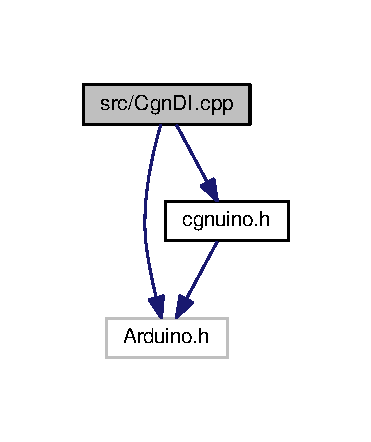
\includegraphics[width=178pt]{CgnDI_8cpp__incl}
\end{center}
\end{figure}


\subsection{Detailed Description}
Definition of \hyperlink{classCgnDI}{Cgn\+DI} class. 

\begin{DoxyAuthor}{Author}
Kei Mochizuki 
\end{DoxyAuthor}

\hypertarget{CgnDO_8cpp}{}\section{src/\+Cgn\+DO.cpp File Reference}
\label{CgnDO_8cpp}\index{src/\+Cgn\+D\+O.\+cpp@{src/\+Cgn\+D\+O.\+cpp}}


Definition of \hyperlink{classCgnDO}{Cgn\+DO} class.  


{\ttfamily \#include \char`\"{}Arduino.\+h\char`\"{}}\\*
{\ttfamily \#include \char`\"{}cgnuino.\+h\char`\"{}}\\*
Include dependency graph for Cgn\+D\+O.\+cpp\+:\nopagebreak
\begin{figure}[H]
\begin{center}
\leavevmode
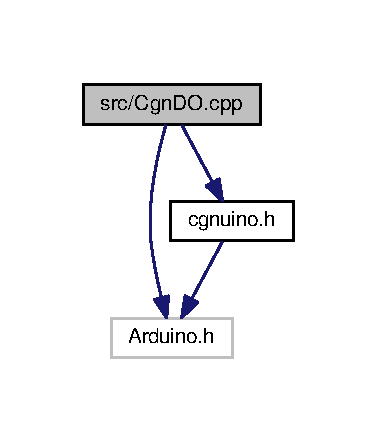
\includegraphics[width=181pt]{CgnDO_8cpp__incl}
\end{center}
\end{figure}


\subsection{Detailed Description}
Definition of \hyperlink{classCgnDO}{Cgn\+DO} class. 

\begin{DoxyAuthor}{Author}
Kei Mochizuki 
\end{DoxyAuthor}

\hypertarget{CgnLogger_8cpp}{}\section{src/\+Cgn\+Logger.cpp File Reference}
\label{CgnLogger_8cpp}\index{src/\+Cgn\+Logger.\+cpp@{src/\+Cgn\+Logger.\+cpp}}


Definition of \hyperlink{classCgnLogger}{Cgn\+Logger} class.  


{\ttfamily \#include \char`\"{}Arduino.\+h\char`\"{}}\\*
{\ttfamily \#include \char`\"{}cgnuino.\+h\char`\"{}}\\*
Include dependency graph for Cgn\+Logger.\+cpp\+:\nopagebreak
\begin{figure}[H]
\begin{center}
\leavevmode
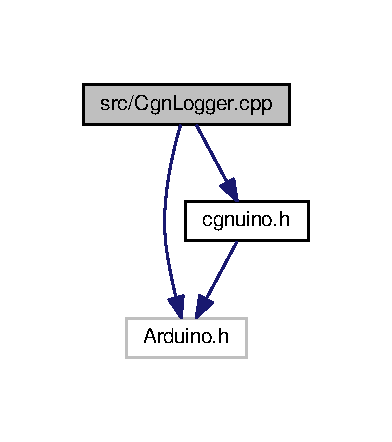
\includegraphics[width=188pt]{CgnLogger_8cpp__incl}
\end{center}
\end{figure}


\subsection{Detailed Description}
Definition of \hyperlink{classCgnLogger}{Cgn\+Logger} class. 

\begin{DoxyAuthor}{Author}
Kei Mochizuki 
\end{DoxyAuthor}

\hypertarget{CgnPause_8cpp}{}\section{src/\+Cgn\+Pause.cpp File Reference}
\label{CgnPause_8cpp}\index{src/\+Cgn\+Pause.\+cpp@{src/\+Cgn\+Pause.\+cpp}}


Definition of \hyperlink{classCgnPause}{Cgn\+Pause} class.  


{\ttfamily \#include \char`\"{}Arduino.\+h\char`\"{}}\\*
{\ttfamily \#include \char`\"{}cgnuino.\+h\char`\"{}}\\*
Include dependency graph for Cgn\+Pause.\+cpp\+:\nopagebreak
\begin{figure}[H]
\begin{center}
\leavevmode
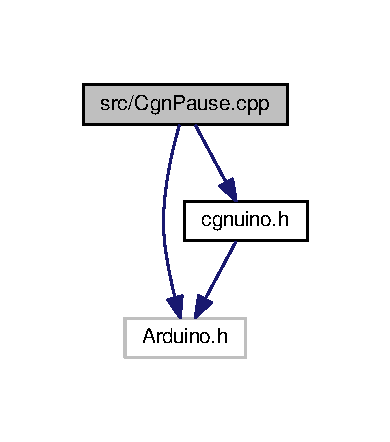
\includegraphics[width=187pt]{CgnPause_8cpp__incl}
\end{center}
\end{figure}


\subsection{Detailed Description}
Definition of \hyperlink{classCgnPause}{Cgn\+Pause} class. 

\begin{DoxyAuthor}{Author}
Kei Mochizuki 
\end{DoxyAuthor}

\hypertarget{CgnPeriod_8cpp}{}\section{src/\+Cgn\+Period.cpp File Reference}
\label{CgnPeriod_8cpp}\index{src/\+Cgn\+Period.\+cpp@{src/\+Cgn\+Period.\+cpp}}


Definition of \hyperlink{classCgnPeriod}{Cgn\+Period} class.  


{\ttfamily \#include \char`\"{}Arduino.\+h\char`\"{}}\\*
{\ttfamily \#include \char`\"{}cgnuino.\+h\char`\"{}}\\*
Include dependency graph for Cgn\+Period.\+cpp\+:\nopagebreak
\begin{figure}[H]
\begin{center}
\leavevmode
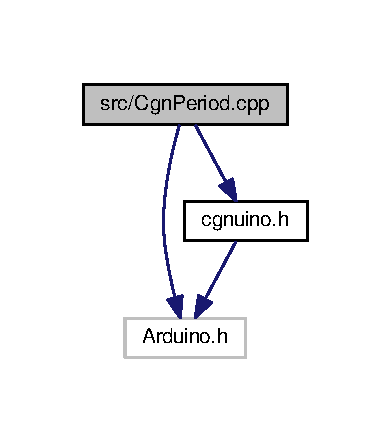
\includegraphics[width=187pt]{CgnPeriod_8cpp__incl}
\end{center}
\end{figure}


\subsection{Detailed Description}
Definition of \hyperlink{classCgnPeriod}{Cgn\+Period} class. 

\begin{DoxyAuthor}{Author}
Kei Mochizuki 
\end{DoxyAuthor}

\hypertarget{CgnSerial_8cpp}{}\section{src/\+Cgn\+Serial.cpp File Reference}
\label{CgnSerial_8cpp}\index{src/\+Cgn\+Serial.\+cpp@{src/\+Cgn\+Serial.\+cpp}}


Definition of \hyperlink{classCgnSerial}{Cgn\+Serial} class.  


{\ttfamily \#include \char`\"{}Arduino.\+h\char`\"{}}\\*
{\ttfamily \#include \char`\"{}cgnuino.\+h\char`\"{}}\\*
Include dependency graph for Cgn\+Serial.\+cpp\+:\nopagebreak
\begin{figure}[H]
\begin{center}
\leavevmode
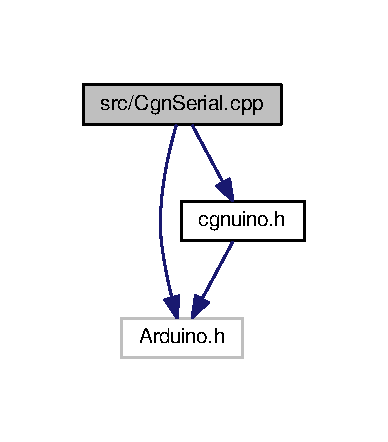
\includegraphics[width=186pt]{CgnSerial_8cpp__incl}
\end{center}
\end{figure}


\subsection{Detailed Description}
Definition of \hyperlink{classCgnSerial}{Cgn\+Serial} class. 

\begin{DoxyAuthor}{Author}
Kei Mochizuki 
\end{DoxyAuthor}

\hypertarget{CgnStopwatch_8cpp}{}\section{src/\+Cgn\+Stopwatch.cpp File Reference}
\label{CgnStopwatch_8cpp}\index{src/\+Cgn\+Stopwatch.\+cpp@{src/\+Cgn\+Stopwatch.\+cpp}}


Definition of \hyperlink{classCgnStopwatch}{Cgn\+Stopwatch} class.  


{\ttfamily \#include \char`\"{}Arduino.\+h\char`\"{}}\\*
{\ttfamily \#include \char`\"{}cgnuino.\+h\char`\"{}}\\*
Include dependency graph for Cgn\+Stopwatch.\+cpp\+:\nopagebreak
\begin{figure}[H]
\begin{center}
\leavevmode
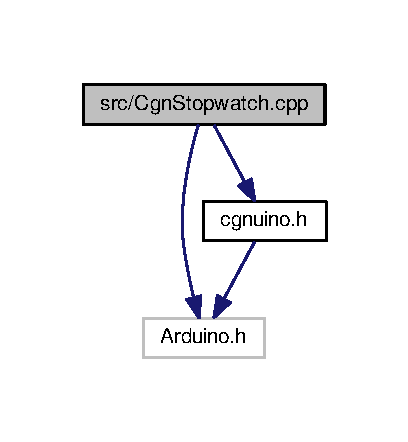
\includegraphics[width=196pt]{CgnStopwatch_8cpp__incl}
\end{center}
\end{figure}


\subsection{Detailed Description}
Definition of \hyperlink{classCgnStopwatch}{Cgn\+Stopwatch} class. 

\begin{DoxyAuthor}{Author}
Kei Mochizuki 
\end{DoxyAuthor}

\hypertarget{CgnStrobe_8cpp}{}\section{src/\+Cgn\+Strobe.cpp File Reference}
\label{CgnStrobe_8cpp}\index{src/\+Cgn\+Strobe.\+cpp@{src/\+Cgn\+Strobe.\+cpp}}


Definition of \hyperlink{classCgnStrobe}{Cgn\+Strobe} class.  


{\ttfamily \#include \char`\"{}Arduino.\+h\char`\"{}}\\*
{\ttfamily \#include \char`\"{}cgnuino.\+h\char`\"{}}\\*
Include dependency graph for Cgn\+Strobe.\+cpp\+:\nopagebreak
\begin{figure}[H]
\begin{center}
\leavevmode
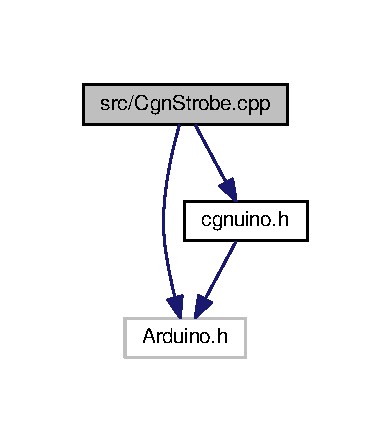
\includegraphics[width=187pt]{CgnStrobe_8cpp__incl}
\end{center}
\end{figure}


\subsection{Detailed Description}
Definition of \hyperlink{classCgnStrobe}{Cgn\+Strobe} class. 

\begin{DoxyAuthor}{Author}
Kei Mochizuki 
\end{DoxyAuthor}

\hypertarget{cgnuino_8h}{}\section{src/cgnuino.h File Reference}
\label{cgnuino_8h}\index{src/cgnuino.\+h@{src/cgnuino.\+h}}


Header file for cgnuino library.  


{\ttfamily \#include \char`\"{}Arduino.\+h\char`\"{}}\\*
Include dependency graph for cgnuino.\+h\+:\nopagebreak
\begin{figure}[H]
\begin{center}
\leavevmode
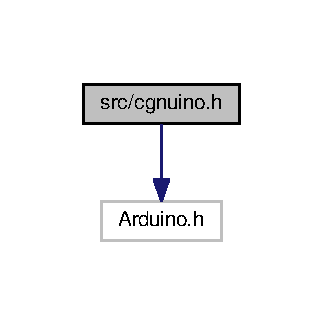
\includegraphics[width=155pt]{cgnuino_8h__incl}
\end{center}
\end{figure}
This graph shows which files directly or indirectly include this file\+:\nopagebreak
\begin{figure}[H]
\begin{center}
\leavevmode
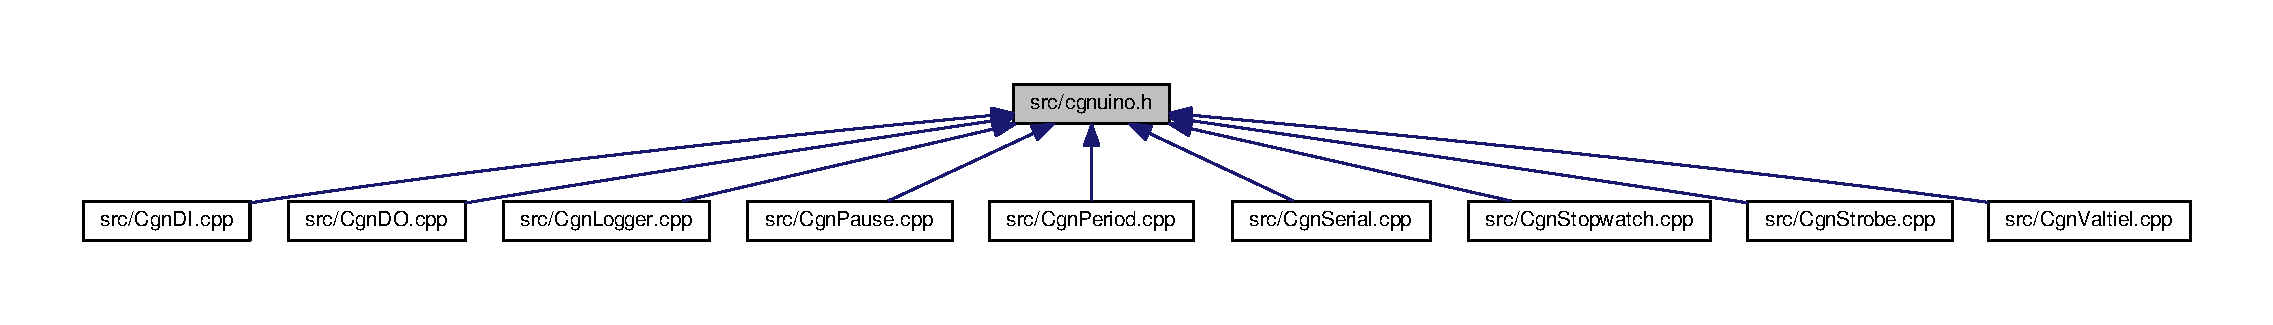
\includegraphics[width=350pt]{cgnuino_8h__dep__incl}
\end{center}
\end{figure}
\subsection*{Classes}
\begin{DoxyCompactItemize}
\item 
class \hyperlink{classCgnDI}{Cgn\+DI}
\begin{DoxyCompactList}\small\item\em Offers convenient digital-\/in buffering. \end{DoxyCompactList}\item 
class \hyperlink{classCgnDO}{Cgn\+DO}
\begin{DoxyCompactList}\small\item\em Emits asynchroneous digital-\/out. \end{DoxyCompactList}\item 
class \hyperlink{classCgnLogger}{Cgn\+Logger}
\begin{DoxyCompactList}\small\item\em Logs arbitorary bit change similar to \hyperlink{classCgnDI}{Cgn\+DI} class. \end{DoxyCompactList}\item 
class \hyperlink{classCgnPause}{Cgn\+Pause}
\begin{DoxyCompactList}\small\item\em Temporally pauses task progression by digital-\/in pin state. \end{DoxyCompactList}\item 
class \hyperlink{classCgnPeriod}{Cgn\+Period}
\begin{DoxyCompactList}\small\item\em Remembers current task period and its time constraint. \end{DoxyCompactList}\item 
class \hyperlink{classCgnSerial}{Cgn\+Serial}
\begin{DoxyCompactList}\small\item\em Communicates with external control apprication running on the PC. \end{DoxyCompactList}\item 
class \hyperlink{classCgnStopwatch}{Cgn\+Stopwatch}
\begin{DoxyCompactList}\small\item\em Measures time difference in milliseconds. \end{DoxyCompactList}\item 
class \hyperlink{classCgnStrobe}{Cgn\+Strobe}
\begin{DoxyCompactList}\small\item\em Emits a text as one-\/by-\/one characters using (8 + 1)-\/bit digital-\/out. \end{DoxyCompactList}\item 
class \hyperlink{classCgnValtiel}{Cgn\+Valtiel}
\begin{DoxyCompactList}\small\item\em Monitors average length of executed loops on Arduino. \end{DoxyCompactList}\end{DoxyCompactItemize}
\subsection*{Macros}
\begin{DoxyCompactItemize}
\item 
\#define \hyperlink{cgnuino_8h_ab317c73e51fb8a68f86165ac831f7b8c}{countof}(array)~(sizeof(array) / sizeof(array\mbox{[}0\mbox{]}))\hypertarget{cgnuino_8h_ab317c73e51fb8a68f86165ac831f7b8c}{}\label{cgnuino_8h_ab317c73e51fb8a68f86165ac831f7b8c}

\begin{DoxyCompactList}\small\item\em Replaced by the length of the array when compiled. \end{DoxyCompactList}\end{DoxyCompactItemize}
\subsection*{Variables}
\begin{DoxyCompactItemize}
\item 
const uint32\+\_\+t \hyperlink{cgnuino_8h_aae502611b08dfc1ddb5ac9a8450150eb}{U\+L\+O\+N\+G\+\_\+\+M\+AX}\hypertarget{cgnuino_8h_aae502611b08dfc1ddb5ac9a8450150eb}{}\label{cgnuino_8h_aae502611b08dfc1ddb5ac9a8450150eb}

\begin{DoxyCompactList}\small\item\em Maximal value for unsigned long. \end{DoxyCompactList}\item 
const byte \hyperlink{cgnuino_8h_a63a8183805bd187b4c3cddf3148ce59c}{B\+Y\+T\+E\+\_\+\+M\+AX}\hypertarget{cgnuino_8h_a63a8183805bd187b4c3cddf3148ce59c}{}\label{cgnuino_8h_a63a8183805bd187b4c3cddf3148ce59c}

\begin{DoxyCompactList}\small\item\em Maximal value for byte. \end{DoxyCompactList}\item 
constexpr byte \hyperlink{cgnuino_8h_ae44d69d4bfcae5aefd4fc3ac732f598a}{N\+\_\+\+C\+G\+N\+DI} = 10\hypertarget{cgnuino_8h_ae44d69d4bfcae5aefd4fc3ac732f598a}{}\label{cgnuino_8h_ae44d69d4bfcae5aefd4fc3ac732f598a}

\begin{DoxyCompactList}\small\item\em Number of pins that can be simultaneously set for a \hyperlink{classCgnDI}{Cgn\+DI} instance. \end{DoxyCompactList}\item 
constexpr byte \hyperlink{cgnuino_8h_adb729e7e1080ed2b4e2872f46a970d15}{N\+\_\+\+C\+G\+N\+DO} = 10\hypertarget{cgnuino_8h_adb729e7e1080ed2b4e2872f46a970d15}{}\label{cgnuino_8h_adb729e7e1080ed2b4e2872f46a970d15}

\begin{DoxyCompactList}\small\item\em Number of pins that can be simultaneously set for a \hyperlink{classCgnDO}{Cgn\+DO} instance. \end{DoxyCompactList}\item 
constexpr byte \hyperlink{cgnuino_8h_af95f44fba5dd40915143e8f9ef8277c6}{N\+\_\+\+C\+G\+N\+V\+A\+L\+T\+I\+EL} = 20\hypertarget{cgnuino_8h_af95f44fba5dd40915143e8f9ef8277c6}{}\label{cgnuino_8h_af95f44fba5dd40915143e8f9ef8277c6}

\begin{DoxyCompactList}\small\item\em Number of buffers \hyperlink{classCgnValtiel}{Cgn\+Valtiel}, speed checker for main loop, can holds. \end{DoxyCompactList}\end{DoxyCompactItemize}


\subsection{Detailed Description}
Header file for cgnuino library. 

\begin{DoxyAuthor}{Author}
Kei Mochizuki 
\end{DoxyAuthor}

\hypertarget{CgnValtiel_8cpp}{}\section{src/\+Cgn\+Valtiel.cpp File Reference}
\label{CgnValtiel_8cpp}\index{src/\+Cgn\+Valtiel.\+cpp@{src/\+Cgn\+Valtiel.\+cpp}}


Definition of \hyperlink{classCgnValtiel}{Cgn\+Valtiel} class.  


{\ttfamily \#include \char`\"{}Arduino.\+h\char`\"{}}\\*
{\ttfamily \#include \char`\"{}cgnuino.\+h\char`\"{}}\\*
Include dependency graph for Cgn\+Valtiel.\+cpp\+:\nopagebreak
\begin{figure}[H]
\begin{center}
\leavevmode
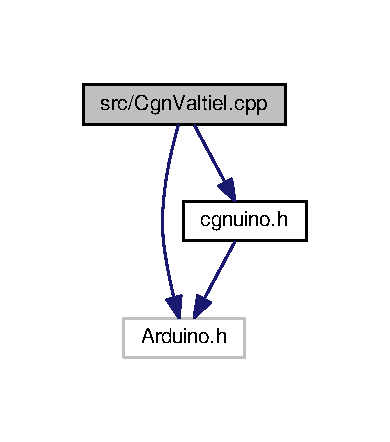
\includegraphics[width=187pt]{CgnValtiel_8cpp__incl}
\end{center}
\end{figure}


\subsection{Detailed Description}
Definition of \hyperlink{classCgnValtiel}{Cgn\+Valtiel} class. 

\begin{DoxyAuthor}{Author}
Kei Mochizuki 
\end{DoxyAuthor}

%--- End generated contents ---

% Index
\backmatter
\newpage
\phantomsection
\clearemptydoublepage
\addcontentsline{toc}{chapter}{Index}
\printindex

\end{document}
